%Subor: prezentace.tex

%Autor: 
%Upravy:

%IFJ11 tim:
%Miroslav Lisik     xlisik00
%Pavol Loffay       xloffa00
%Dusan Madarka      xmadar01
%Fridolin Pokorny   xpokor32

%documentclass
\documentclass[pdf,fyma2,total]{prosper}
%packages
\usepackage[utf8]{inputenc}
\usepackage[slovak]{babel}
\usepackage{picture}
\usepackage{graphics}
\usepackage{multicol}

%prechody slajdov
\DefaultTransition{Replace}
%spodna lista slajdov
\slideCaption{Projekt IFJ 2011}

\begin{document}

\begin{titlepage}
  \title{Projekt IFJ 2011}
  \subtitle{Tím 106, varianta b/1/II}
  \author{Fridolín Pokorný, Pavol Loffay, Dušan Maďarka, Miroslav Lisik}
  \date{\today}
  \maketitle
\end{titlepage}

%%%%%%%%%%%%%%%%%%%%%%%%%%%%%%%%%%%%%%%%%%%%%%%%%%%%%%%%%%%

\begin{slide}{Obsah}
\begin{small}

    \medskip
    \begin{enumerate}
        \item{Implemetácia}
            \begin{enumerate}
                \item[1.1]{Štruktúra intepreta}
                \item[1.2]{Tabuľka symbolov}
                \item[1.3]{Volanie podprogramu}
            \end{enumerate}

        \item{Práca v tíme} 
            \begin{enumerate}
                \item[2.1]{Rozdelenie úloh a metodiky}
                \item[2.2]{Štatistiky}
            \end{enumerate}

        \item{Záver}

        \item{Diskusia}

    \end{enumerate}

\end{small}
\end{slide}

%%%%%%%%%%%%%%%%%%%%%%%%%%%%%%%%%%%%%%%%%%%%%%%%%%%%%%%%%%%

\begin{slide}{Štruktúra intepreta}
\begin{small}

    \bigskip
    \begin{itemize}
        \item{lexikálny analyzátor\,--\,konečný automat}
        \bigskip
        \item{syntaktický analyzátor\,--\,rekurzívny zostup}
        \bigskip
        \item{vyhodnocovanie výrazov\,--\,precedenčná analýza}
        \bigskip
        \item{interpret spracováva trojadresný kód}
    \end{itemize}

\end{small}
\end{slide}

%%%%%%%%%%%%%%%%%%%%%%%%%%%%%%%%%%%%%%%%%%%%%%%%%%%%%%%%%%%

\begin{slide}{Tabuľka symbolov}
\begin{multicols}{2}

    \begin{small}
        \begin{itemize}
            \item{tabuľka\\s~rozptýlenými položkami (TRP)}
            \medskip
            \item{položkou tabuľky je záznam o~funkcii}
            \medskip
            \item{obsahuje názov, zoznam\\inštrukcií, počet parametrov a\\zoznam
            premenných}
        \end{itemize}
    \end{small}
    \bigskip
    \begin{center}
        \begin{figure}[h!]
            \scalebox{0.2}{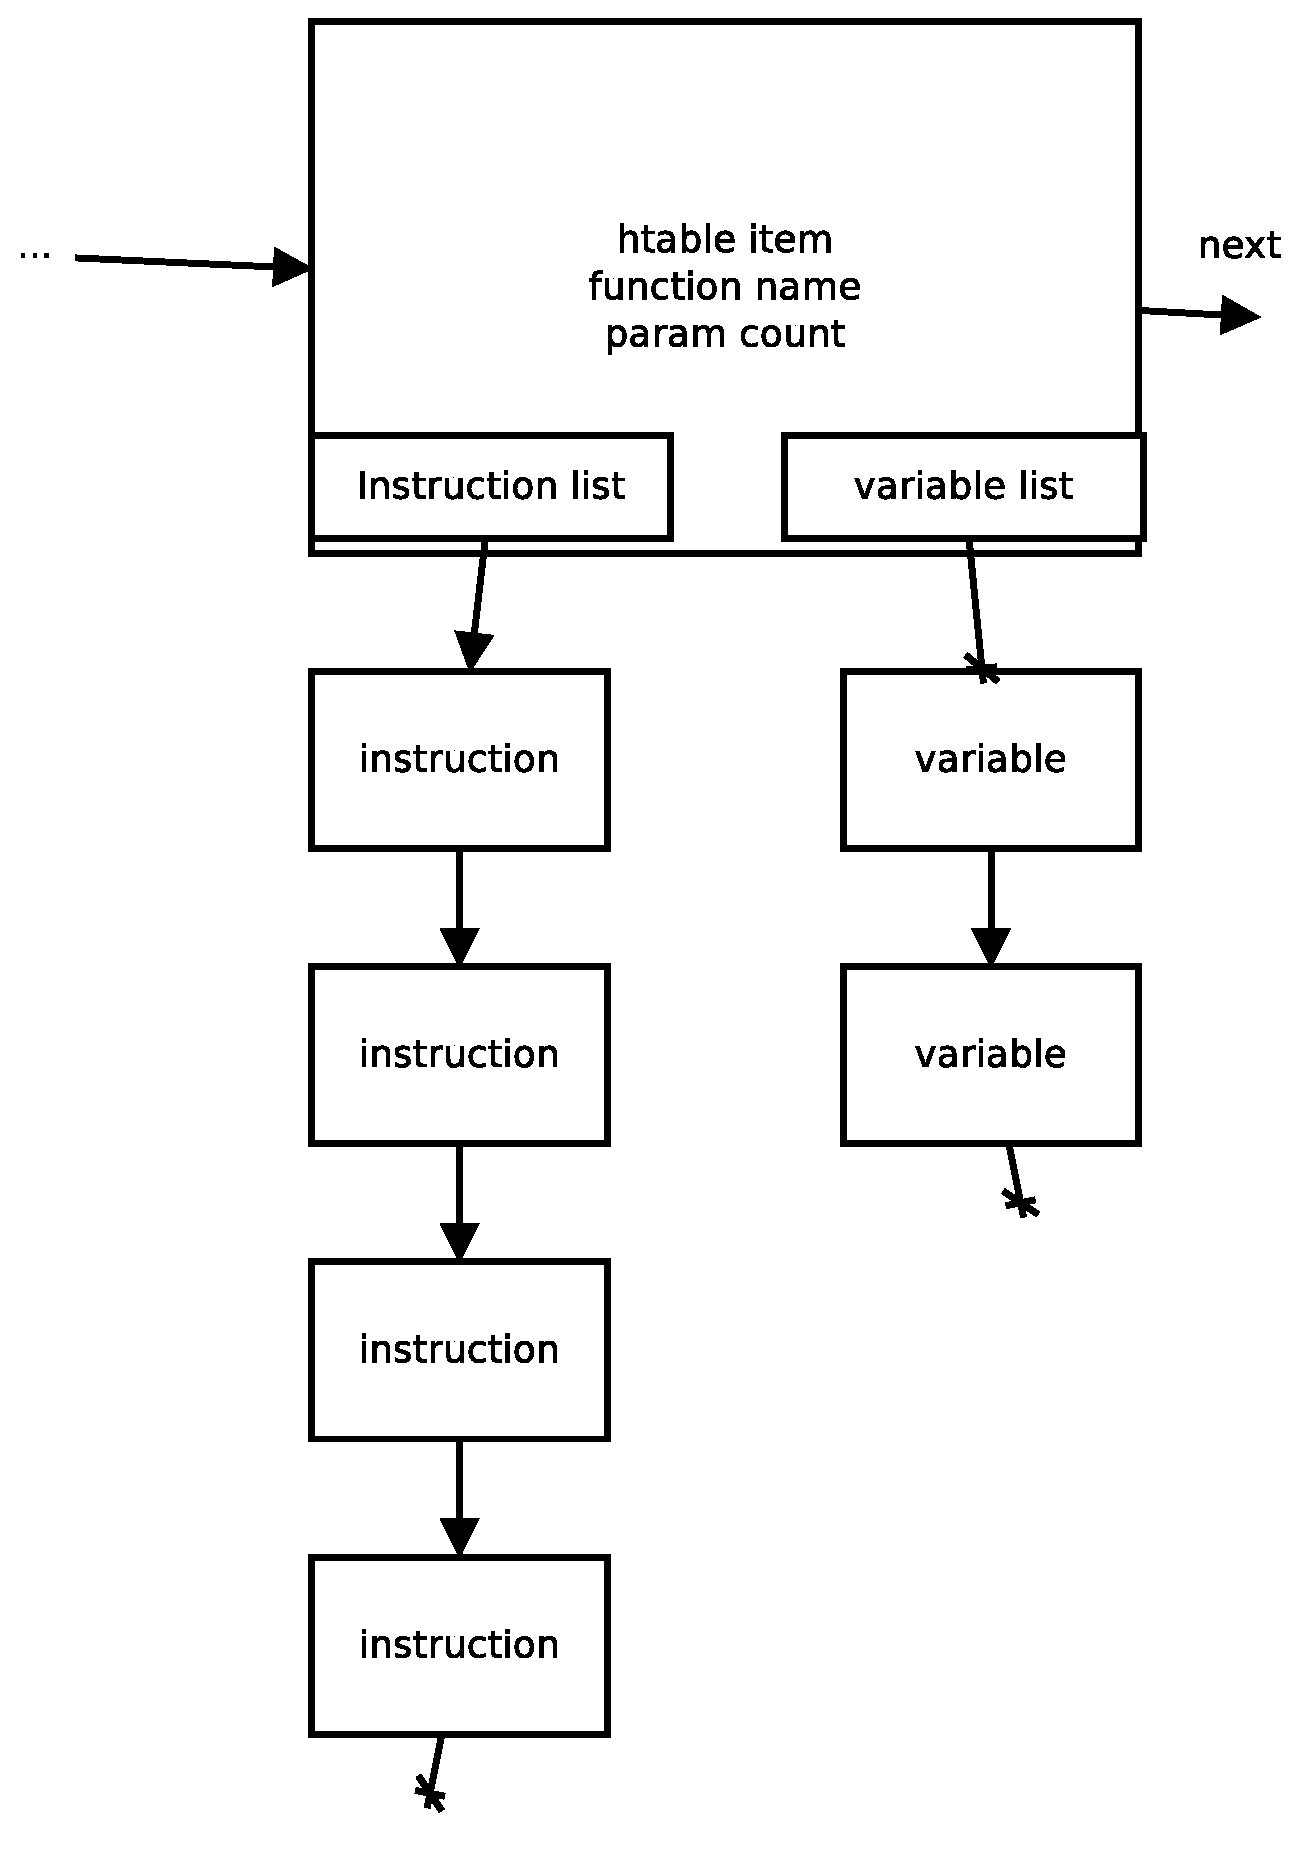
\includegraphics{img/htable_item.eps}}
            \caption{\small{položka TRP}}
            \label{int-obr1}
        \end{figure}
    \end{center}

\end{multicols}
\end{slide}

%%%%%%%%%%%%%%%%%%%%%%%%%%%%%%%%%%%%%%%%%%%%%%%%%%%%%%%%%%%

\begin{slide}{Programový zásobník}
    \begin{small}
        \begin{itemize}
            \item{predávanie argumentu, záloha premenných a návrat}
        \end{itemize}
    \end{small}

    \begin{figure}[h!]
    \begin{center}
        \scalebox{0.18}{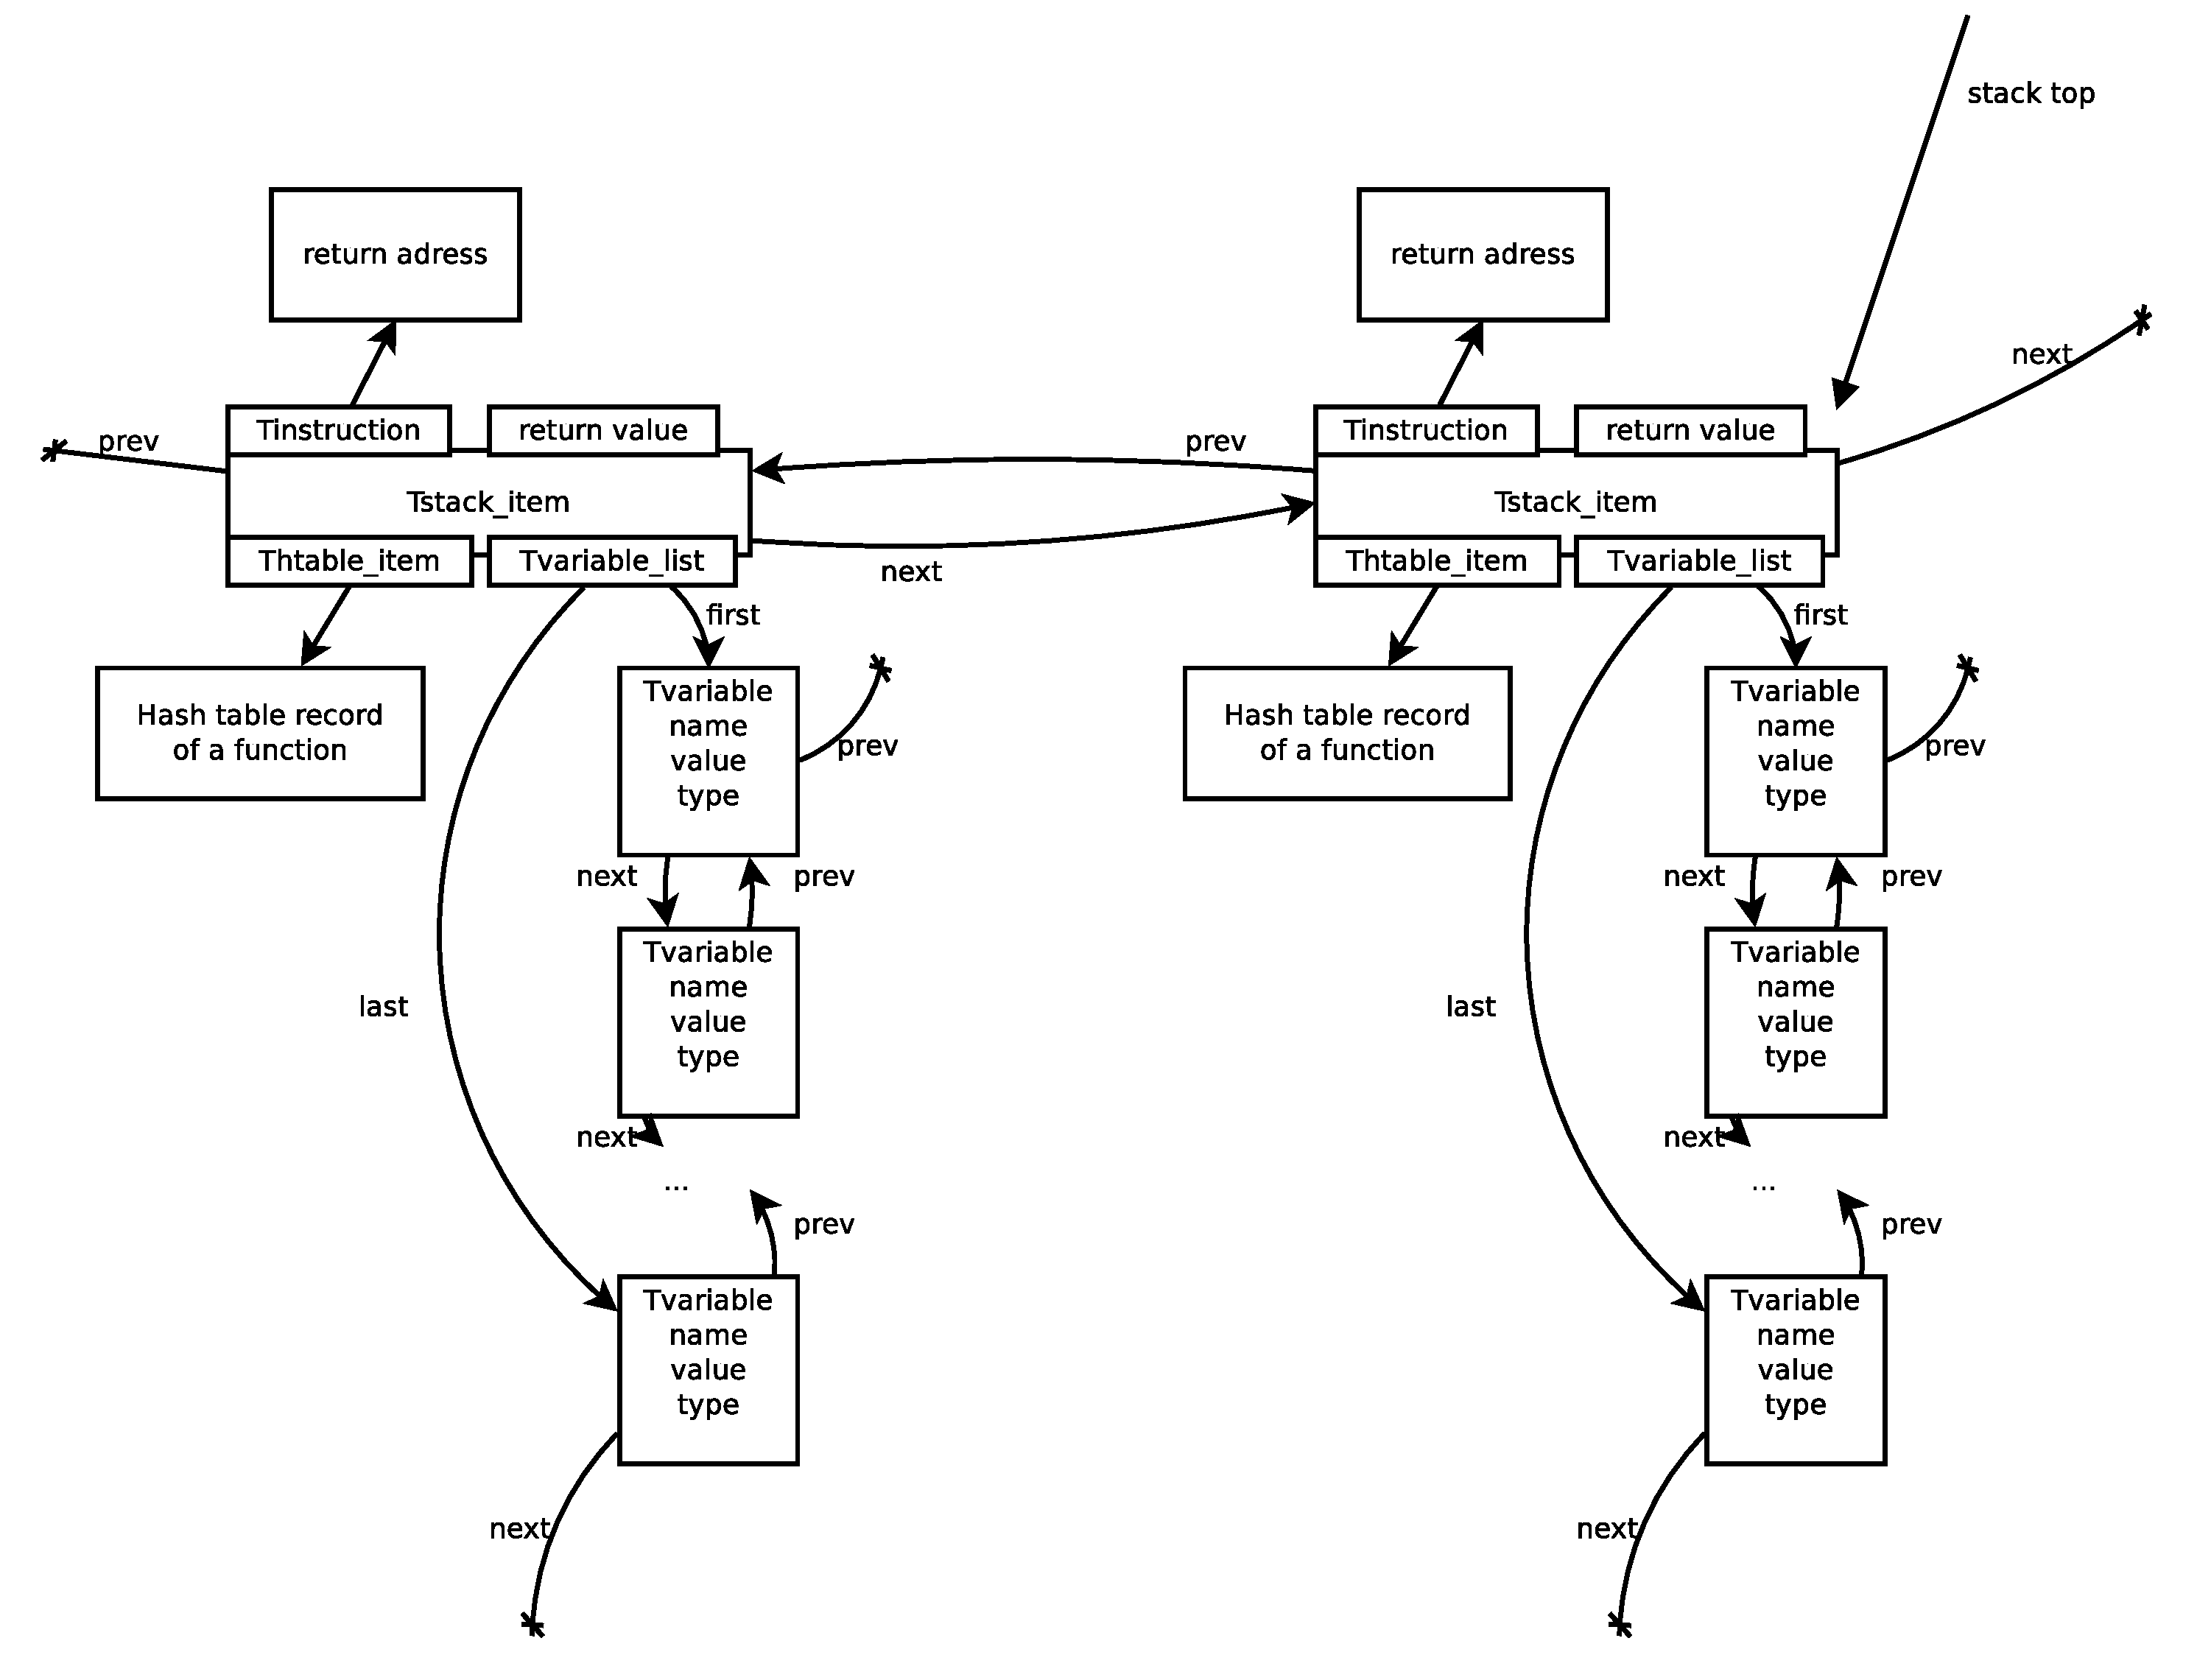
\includegraphics{img/call_stack.eps}}
    \end{center}
    \end{figure}
\end{slide}

%%%%%%%%%%%%%%%%%%%%%%%%%%%%%%%%%%%%%%%%%%%%%%%%%%%%%%%%%%%

\begin{slide}{Rozdelenie úloh a metodiky}
\begin{small}

    \bigskip
    \begin{itemize}
        \item{určenie zodpovedných za sekcie}
        \bigskip
        \item{každý člen tímu sa podieľal aj na ostatných častiach}
        \bigskip
        \item{dôraz na komunikáciu}
        \bigskip
        \item{pravidelné osobné schôdze}
        \bigskip
        \item{verzovací systém Subversion, Redmine}
        \bigskip
        \item{špecifikácia testov pred implemetáciou}
    \end{itemize}

\end{small}
\end{slide}

%%%%%%%%%%%%%%%%%%%%%%%%%%%%%%%%%%%%%%%%%%%%%%%%%%%%%%%%%%%

\begin{slide}{Štatistiky 1/2}

    \begin{center}
        \begin{figure}[h!]
            \scalebox{1.5}{\includegraphics{img/statis1.eps}}
            \caption{\small{Počet riadkov kódu vzhľadom na dátum.}}
            \label{int-obr1}
        \end{figure}
    \end{center}

\end{slide}

%%%%%%%%%%%%%%%%%%%%%%%%%%%%%%%%%%%%%%%%%%%%%%%%%%%%%%%%%%%

\begin{slide}{Štatistiky 2/2}
    \begin{center}
        \begin{figure}[h!]
            \scalebox{1.5}{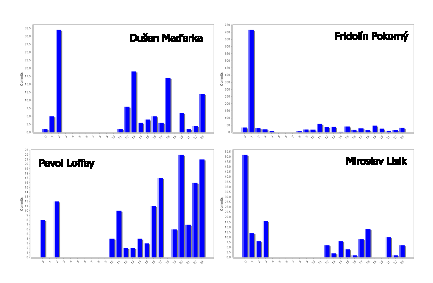
\includegraphics{img/statis2.eps}}
            \caption{\small{Aktivita členov počas dňa.}}
            \label{int-obr2}
        \end{figure}
    \end{center}
\end{slide}

%%%%%%%%%%%%%%%%%%%%%%%%%%%%%%%%%%%%%%%%%%%%%%%%%%%%%%%%%%%

\begin{slide}{Záver}
\begin{small}
    \bigskip
    \begin{itemize}
        \item{objasnenie zložitosti prekladačov a~interpretov}
        \medskip
        \item{náročnosť zotavovania z chýb, optimalizácie}
        \medskip
        \item{prípadné zmeny do budúcna:}
        \begin{itemize}
            \medskip
            \item{aktivita zoznamu inštrukcií\,--\,rozšírenie \texttt{FORDO}}
        \end{itemize}
    \end{itemize}
\end{small}
\end{slide}

%%%%%%%%%%%%%%%%%%%%%%%%%%%%%%%%%%%%%%%%%%%%%%%%%%%%%%%%%%%

\begin{slide}{Diskusia}
    \begin{center}
            \bigskip
            \bigskip
            \bigskip
            \bigskip
            \bigskip
            \bigskip
            {\Large ?}{\Huge ?}{\Large ?}
            \bigskip
            \bigskip
            \bigskip
            \bigskip
            \bigskip
            \bigskip
            \bigskip
            \bigskip
    \end{center}

    \begin{flushright}
        Ďakujeme za pozornosť a vidíme sa na skúške.
    \end{flushright}
\end{slide}

%%%%%%%%%%%%%%%%%%%%%%%%%%%%%%%%%%%%%%%%%%%%%%%%%%%%%%%%%%%

\end{document}
